% !TeX root = ../main.tex
% %%%%%%%%%%%%%%%%%%%%%%%%%%%%%%%%%%%%%%%%%%%%%%%%%%%%%%%%%%%%%%%%%%%%%%%%%%%%%%
% Introduction
\chapter{Introduction}
\label{chap:introduction}

Robotics already have a great impact in our current society so, 
the quality of software used by robots should be of extreme importance for us.
Robot software as well as the techniques used to test their quality are 
very specific to the field and differ a lot from the norm.
Automatic tests are barely used in robotics due to multiple factors.
The intention is then to create a tool that will promote the safe 
and reliable execution of automatic tests.
This tool will contemplate both a descriptive high-level language 
that should capture certain properties of a robot and a way to create test scenarios.

% ------------------------------------------------------------------------------
% Motivation
\section{Motivation}
\label{sec:motivation}

Currently, robots are vastly used industrially (medicine, agriculture, etc.) 
or as a form of leisure (contests, personal use, etc.).
The tendency is for robot usage to keep growing at a global level.
Robot tasks tend to be repetitive and/or rather specific.
Robot software also tends to be quite different from conventional software.
The Cyber-Physical systems of robots are non-deterministic and unreliable.
One reason is the fact that robots interact directly with their environment.
A sensor can return imprecise values since the environment itself can be very hard to predict.
As a result, the notion that a task or movement is correct is really hard for a robot to conceive.

\par

\alcides{Falas em testes automáticos, mas deverias primeiro identificar soluções para evitar isto. Introduzir primeiro testes, depois testes automáticos.}

Consequentemente testes 
automáticos são difíceis de realizar nesta área, de facto atualmente a grande maioria dos testes 
realizados em robôs necessitam de supervisionamento humano seja o teste feito no mundo real ou numa 
simulação, identifica-se assim que existe um espaço para melhoramento na área de testes para robôs 
através de testes automáticos optimizados com o objectivo de melhorar a qualidade destes sistemas.

\section{Problem Statement}
\label{sec:problem}

There are multiple challenges in robot testing, costs, 
complexity, hardware integration, among others.
When planning on how to test a robot there are tradeoffs between the 
different choices to make given into account all the challenges.
While tests using simulations are a promising approach for automation 
there is still distrust in the precision and validity of the results.
This means, although dangerous and sometimes expensive real-life 
robot testing is still the prime choice.
Be the tests done in the real world or resorting to simulation, 
human supervising will most likely still be necessary.
This is because identifying if a robot fulfills an expected 
behavior is really hard for the robot itself.
For this reason, automatic tests in the robotics field are 
hardly reliable and hard to implement.
The resulting product is a lack of quality in the software across projects~\cite{TestRob}.

% ------------------------------------------------------------------------------
% Objectives
\section{Objectives}
\label{sec:objectives}

\alcides{A primeira frase tem de ser reescrita. Não facilitas developers, mas facilitas a criação de testes automáticos.}
Este trabalho tem como objectivo dar a mostrar o potencial de testes automáticos em robótica e facilitar 
developers do ramo na realização de testes nos seus robôs. Para atingir este objectivo propõe-se criar 
um mecanismo de monitorização de certos componentes do robô durante e/ou após a execução de um teste. 


\alcides{Queres arbitrários em vez de aleatórios. Acho que devias começar com o desenho de uma linguagem de alto nível para especificação de propriedades de sistemas robóticos. Depois um compilador que traduzia essa linguagem num mecanismo de monitorização. Mas a linguagem devia ser o ponto inicial. Acho que falar do GZScenic ainda não é relevante aqui.}
Estes componentes do robô não serão aleatórios mas sim definidos com a ajuda de uma nova linguagem de 
alto nível, o objectivo é conseguir-se descrever as propriedades do robô com ajuda desta linguagem, 
deste modo se o robô não seguir as propriedades definidas durante um teste o seu comportamento não será 
correcto. Será também preciso criar cenários de teste específicos e aleatórios para o robô de uma forma 
automática, já existindo uma linguagem para este efeito (GzScenic)~\cite{GzScenic} pode-se tirar partido 
da mesma.
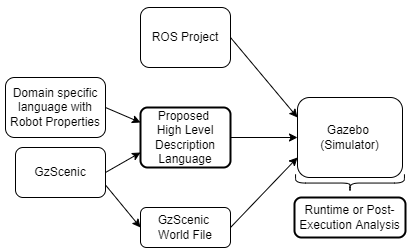
\includegraphics{images/intro_diag.png}
\alcides{A imagem devia estar como uma figura. A parte do GzScenic ainda não é relevante. Falta uma legenda dos vários tipos de componentes da imagem.}
\alcides{Neste ponto ainda não apresentaste o ROS. Acho relevante dar uma pequena introdução ao que é, para se perceber aqui o esquema.}

\section{Contributions}
\label{sec:contributions}

The expected contributions of this thesis are below enumerated.

Alterar a prespectiva da utilização de testes automáticos na área da robótica.

Criar uma ferramenta simples de usar que permite realizar testes automáticos na área da robótica.


\alcides{Aqui pretendem-se coisas mais concretas: 1. Definição de uma linguagem de alto nível para especificação de propriedades de robots. Depois um compilador dessa linguagem para monitorização. Depois uma avaliação da capacidade desta solução modelar vários problemas relevantes na robótica.}

% ------------------------------------------------------------------------------
% Structure of the document
\section{Structure of the document}
\label{sec:structure}

The document is organized as follows:

\begin{itemize}
    \item Section 1...
    \item Section 2...
    \item Section 3...
\end{itemize}

